%!TEX root = project.tex

\chapter*{About this project}

\paragraph{Abstract}


\paragraph{Authors}


\chapter*{Acknowledgements}


\chapter{Introduction}

When choosing our project we wanted to pick something that was relevant to current everyday life. We wanted a project that also highlighted our skills and allowed us to learn and develop as part of a team. With this criteria in mind we started brain storming ideas for our project.

We eventually decided on a App called Digs. Digs would be a Student Accommodation app. We recognized the current accommodation crisis throughout Ireland and thought it would benefit students and landlords to have a specific letting app for the student population. Also for students it was quiet disheartening to apply for accommodation and be rejected for being of student status. This is quiet common when renting and with our app they would only be applying for lettings specific to them.

Having a student accommodation app as our starting point we started to research other apps and websites in the accommodation letting/renting category. The main one we focused on was the Daft App\cite{Daft}. Daft would be the most popular accommodation app in Ireland and it provided us with a great deal of insight on what our app would need to have and also on what Daft lacks for the student market. 

We wanted a app that had essentially the same functionality as Daft but which was geared more towards student. We did this by focusing on the college campuses and not specific cities. We also created a forum for students to get in touch with one another, to either get a house together or to get someone for a room in the house they are already renting. These would compliment the normal functionality of a accommodation app such as, publish ads (either rooms or properties), search lists (rooms or properties), view rooms and properties and edit and delete your personal ads. This would also require log in and registration functionality.

After deliberating over the objective of our application, we then turned to what technology we would use. We wanted to use a array of technologies to show our capabilities but also gain more knowledge and become better programmers over all. We settled on a 3 tier structure containing a Ionic 3 presentation tier(front end), NodeJs logic tier(middleware)  and Mongo/firebase database data tier(back end).

From what we hoped to achieve from creating this app was the knowledge of new technology, personal growth through team building and of course to produce something of substance and something we could be proud of.

\chapter{Context}
The general context of our application resolves around students having a platform which is geared towards finding accommodation. Students will be able to search through available listings, advertise their own rooms for rent and allows letters to advertise full properties to students. Listings can be created by advertising a room or property, with a series of criteria. Some examples of criteria would be proximity to College campus, room/property type, location, price, contact information and a description. Along with this information, images can be taken with the user’s device camera or uploaded directly from their device which is then linked with that listing. Students looking for accommodation can also search through available listings based on the following criteria: 

\begin{itemize}
  \item Price
  \item Which college campuses are close
  \item Room/Property Type
  \item Parking Availability
\end{itemize}

\section{Objectives}
The main objective of our application is to help students who may be struggling with the current accommodation crisis in Ireland. We also wanted to make it easier for students and landlords, who are looking to rent or let. The following is a list of the main pages in our application along with the objectives for each page. 

\begin{enumerate}
    \item \textbf{Login/Register Page} Our application has a login and a register page. The following are the objectives for these pages. The register page allows the user to securely register with our application while the login page allows the user to securely login to our application. Once logged in the user has access to extra features not accessible to unregistered users. 
    
    \item \textbf{Forgot-Password Page}
    The objective of the forgot-password page is to allow a user who has forgotten their password to enter their email address. They will then receive an email containing a link which will allow them to create a new password.

    \item \textbf{Home Page} 
    The objective of the homepage is that it is a base of navigation for the application. It displays the total number of both properties and rooms that are currently listed. The homepage will also display if a user is logged in or not.
    
    \item \textbf{List of Rooms/Properties Page} 
    The objective of both these pages is to display all the currently listed rooms and properties to the user. Showing the main criteria on each room/property so the user can make an informed decision.
    
    \item \textbf{Create a Room/Property Page} 
    The objective of both these pages is to allow the user to create a room or property listing and then publish it. This will allow the user to showcase their room/property using images, filling in form details and their own personal description.
    
    \item \textbf{Message Board} 
    The objective of the message board is to have a place where students can communicate with each other, helping themselves find other students that are looking for accommodation
    
    \item \textbf{Search} 
    The objective of the search page is to allow students to refine the number of listings based upon criteria they specify. 
    
    \item \textbf{My Ads Page}
    The objective of the My Ad’s page is to allow a user to view a list of their published ads. In here they can delete these ads or they have the option to edit their published ads.
\end{enumerate}

\section{Project Links}
Below are the links for our project. They include the URL link to our GitHub repository and the URL link to our Dissertation.

\paragraph{Link to Repository}
\begin{itemize}
\item \href{https://github.com/gerardnaughton7/4th-Year-Final-Year-Project}{https://github.com/gerardnaughton7/4th-Year-Final-Year-Project} 
\end{itemize}

\paragraph{Direct Link to Dissertation Pdf}
\begin{itemize}
    \item \href{https://github.com/gerardnaughton7/4th-Year-Final-Year-Project/tree/master/DigsDissertation/}{https://github.com/gerardnaughton7/4th-Year-Final-Year-Project/tree/master/DigsDissertation/}
\end{itemize}

\section{Chapters Review}
Description of chapters

\subsection{Methodology}
Description of chapters

\subsection{Technology Review}
Description of chapters

\subsection{System Design}
Description of chapters

\subsection{System Evaluation}
Description of chapters

\subsection{Conclusion}
Description of chapters


\chapter{Methodology}
Description of chapters....

\section{Agile Development}
During the life-cycle of our project we attempted to use an Agile like approach to the research, design and implementation stages of the project. In the initial stages of the project we discussed various methodologies we could use, for example Waterfall but we decided on Agile. This is because Agile offers continual improvement, flexibility and incremental delivery of the software. \\

\noindent During the research process of our project we used a Scrum like approach. Scrum is an Agile method in which a development cycle is carried out in what are known as sprints. \\

\noindent During the development process of our Digs application we used a RAD like approach. RAD, Rapid Application Development, is an agile approach to software development which puts less emphasis on planning and more emphasis on actual development. \\

\noindent The following section contains information about the various sprints we undertook in the research cycle of our project.

\section{Sprints}
Each of the sprints we completed during our research and planning phase of our project gave us, as a team, the opportunity to learn and adapt to the various needs of the project. Each sprint represents a vital aspect of the application i.e. Creating three tier architecture, accessing native phone capabilities through Cordova and learning how to integrate all these features together. We prioritised the sprints in the order as follows.

\subsection{Sprint 1 Review King}
This was our first sprint and it was worked on by all three members in our team. Review King is an application we found on a blog by Josh Morony \cite{ReviewKing} in which he explains the process of building a simple review app using three tier technology. On the front end a user can write a small review and then add a score. That information is then sent to a node server which stores the information in a MongoDB database.  We felt it was very important that all three members understood the process involved in connecting these three layers together so we all worked on this sprint together.  

\subsection{Sprint 2 Image Gallery}
This was a relatively small sprint and was completed by Patrick. The plan for this sprint was to create a small app which displayed images in a gallery style format. Using a plugin for ionic called ionic-img-viewer \cite{ImgViwer} an image is made larger when it is clicked. Images can be moved left and right in a gallery style and incorporate zoom functionality.

\subsection{Sprint 3 Image Back-end}
The next phase of the project was figuring out a way of using a mobile devices camera to take a picture, upload that picture to a node server and then save a reference to that image in a MongoDB database. To do this we split this process up into two sprints. The first sprint involved setting up the back end. We achieved this functionality by following a blog by Devdactic \cite{ImageBackEnd} where we set up our NodeJS back-end. Once completed our backend had the capability to upload and store images. This functionality was tested using software called Postman \cite{Postman}. Postman is a HTTP client service which helps developers test their API with various HTTP requests. \\

\subsection{Sprint 4 Image Front-End}

\subsection{Sprint 5 Login/Register}

\noindent The following section contains information about the RAD appraoch we undertook during the development phase of our Digs.

\chapter{Technology Review}

\section{Database}

\subsection{NoSQL database}
The ascent of Big Data made an interest for on a horizontally adaptable Data Management System. This prompted advancement of various types of Database Management System which all things considered go under NoSQL. NoSQL Databases are comprehensively separated into following sorts: Document, Key-value, Graph, Native object, Table type, Native XML and Hybrid Databases. All RDBMS databases depend on the same model, while, each of the NoSQL database takes after a distinctive model. NoSQL moves far from the robust institutionalized type of SQL database and empowers less complex information capacity arrangements. Therefore a NoSQL database is enhanced for the particular application.\cite{noSql}

\subsubsection{NoSql database types}

\begin{itemize}
\item Key-Value Storage \par
Key-Value Storages are straight forward and simple NoSQL frameworks, for example, Redis that are fundamentally a truly favour hash table. You have an esteem you need to get later, so you allocate it a key and in addition stuff it into the database, you can just inquiry a single object at any given moment and just by a single key.

\item Document Storage \par
Regularly, these are objects with a various levelled structure, for example, XML documents, JSON records, and some other kind of tree structure, yet the qualities of various nodes on the tree can be indexed. They have a much speed with respect to customary push construct SQL databases in light of query in light of the fact that they give up execution on joining. 

\item Columnar Storage  \par
These store the information in columns instead of lines, so refreshing and adding are costly, be that as it may, most questions are modest in light of the fact that each segment is basically certainly recorded. In any case, on the off chance that your inquiry can not utilize an index, you are in no better shape with a Columnar Store rather than a standard SQL database.

\item Graph Storage  \par
Diagram Databases (neo4j) make joins as shoddy as could be expected under the circumstances, on the grounds that even a straightforward row query would require many joins to recover. Tables can sort query would be slower than a standard SQL database in view of the greater part of the additional joins to retrieve the information. \cite{DataTypes}
\end{itemize}

\subsubsection{Advantages of NoSql}
NoSQL databases are very versatile, dependable, have a basic data model, amazingly exposed query language, no system for taking care of consistency and trustworthiness among data, and no help for security at the database level. A standout amongst the most vital points of interest of NoSQL databases is that the databases can handle unstructured information. Unstructured data can be word reports, messages, sound, video, or even interpersonal social network information. Too, NoSQL databases tend to scale extremely well on commodity equipment. Some even claim that NoSQL databases empower better execution, which is urgent for organizations with a lot of data. To empower quicker execution, NoSQL databases ordinarily don't cling to ACID (atomicity, consistency, isolation, durability) restrictions that are utilized as a part of relational databases. While this is recorded as a star for NoSQL as far as execution and processing time; we take note of that this likewise has unfortunate outcomes that will be tended to later. A case of NoSQL database's execution is Facebook's usage (Cassandra) that is equipped for dealing with more than 100 million clients persistently. \cite{AdvantagesnoSql}

\subsection{Examples of NoSQL}
\begin{itemize}
\item Key-Value Storage: \par
MUMPS, CouchDB, FoundationDB, Redis, Aerospike, Dynamo, MemcacheDB, Riak, OrientDB, Fair Com c-treeACE, Redis.

\item Apache CouchDB, MarkLogic, OrientDB, Clusterpoint, Couchbase, MongoDB.

\item Columnar Storage:  \par
Vertica, Cassandra, Hbase, Accumulo, Druid.

\item Graph Storage:  \par
Neo4J, OrientDB, Stardog, Allegro, InfiniteGraph, Virtuoso. 
\end{itemize}

\subsection{MongoDB}
MongoDB is a cross-platform, document-oriented database that provides high performance and easy scalability. The basis of this database is the concept of collections and documents.\par
MongoDB is ideal for projects that involve working with very large amounts of data and / or high scalability requirements, high performance even in cases where information is too complex and heterogeneous for modeling using a relational schema, or there is a need for real-time analysis \par
In comparison, the contents of a relational database are tables, the MongoDB database consists of collections. Each collection has its own unique name - an arbitrary identifier consisting of no more than 128 different alphanumeric characters and an underscore.
Unlike relational databases, MongoDB does not use a table with data types. MongoDB is a document-oriented system in which the central concept is a document. \par
A document can be represented as an object storing some information. In a sense, it is like strings in relational DB, where lines store information about the element. \cite{MongoDB} \par For example, a typical document:

\begin{minted}{js}
	{
    "name": "Andrei",
    "surname": "Petruk",
    "age": "40",
    "college": {
        "name" : "GMIT",
        "year" : "2018",
        }
}
\end{minted}

\subsubsection{Document ID}
For each document, a unique identifier called id is defined in MongoDB. When you add a document to the collection, this ID is automatically generated. However, the developer can explicitly set the identifier, rather than relying on the automatically generated ones, specifying the corresponding key and its value in the document.\par
This field must have a unique value within the collection. And if we try to add two documents with the same identifier to the collection, we will get an error.\par
If the identifier is not specified explicitly, then MongoDB creates a special binary value of 12 bytes.\cite{MongoDBID}

\subsection{Firebase Authentication}
The authentication service closely integrates with other Firebase services, uses industry standards such as OAuth 2.0 and OpenID Connect, so it can be easily integrated with your backend.\par
The Firebase Authentication SDK provides methods for creating and managing users who use e-mail addresses and passwords to log on to the system.\par
According to the documentation, the listener receives notifications in the following situations:
\begin{itemize}
\item When the FirebaseAuth object completes the initialization and the user is already authorized in the previous session or is redirected from the input stream of the other authentication provider.
\item When the user logs in (the current user is installed)
\item When the user exits (the current user becomes null)
\item When the access token of the current user is updated. This can happen in the following cases:
if the token expired
\item The user re-authenticates
\item The user changes his password.
\end{itemize}
In this case, Firebase issues new access tokens and marks the old ones as invalid. When changing the password, the user logs off automatically on each device, for security reasons. \cite{Firebase}

\section{Server}

\subsection{NodeJS}
Node or Node.js is a software platform based on the V8 engine (translating JavaScript into machine code), which turns JavaScript from a highly specialized language into a general-purpose language. Node.js adds the ability of JavaScript to interact with I / O devices through its API (written in C ++), connect other external libraries written in different languages, providing calls to them from JavaScript code. Node.js is used primarily on the server, acting as a web server, but it is possible to develop Node.js and desktop window applications (using NW.js, AppJS or Electron for Linux, Windows and Mac OS) and even program microcontrollers (for example, tessel and espruino). Node.js is based on event-oriented and asynchronous programming with non-blocking I / O. \par 
An important thing to realize is that Node is not a web server. The platform itself does not do anything. It does not work like Apache. There are no configuration files in which it points you to HTML files. If you want the platform to be an HTTP server, you'll have to write an HTTP server (using built-in libraries).
\cite{NodeJS}

\subsubsection{Asynchronous calls}
Asynchronous calls are especially important for web servers. It is quite typical for modern web applications to have access to databases. While waiting for the result to return from the database, Node can process more queries. This allows you to cope with thousands of parallel requests with little overhead compared to creating a separate thread for each connection. \cite{NodeJS}

\subsubsection{npm}
Node.js Package Manager is the package manager that is part of the Node.js.
Now, instead of installing each library separately, we can run one command and install everything in one go.

\begin{minted}{js}
npm install
\end{minted}

When you run the command, npm will look for the package.json file in the current folder. If found, it will install each library from the list. \cite{NodeJS}

\section{Front End}

\subsection{Ionic}
Ionic is a framework with a stunningly designed graphical interface, styled for various platforms, for maximum similarity to native applications. AngularJS and sass are taken as a basis for the framework, which brought him great popularity among developers, as these technologies reduce the threshold of entry to a minimum. The core of the framework is Cordova, so all the plugins of Cordova will work fine on ionic.\par In addition to the platform and ready-made UI components, Ionic has a thoughtful command line interface that allows you to generate icons, splash screens, run the file in the browser with the app for debugging, and build applications with short commands in the console.\par Also worth noting is the detailed documentation with examples.\cite{Ionic}

\subsubsection{Ionic UI}
Ionic has dozens of ready-made components, which are constantly being refined and replenished with new ones. You can fully read them on the documentation page.\cite{IonicUI}

\begin{figure}[h]
\centering
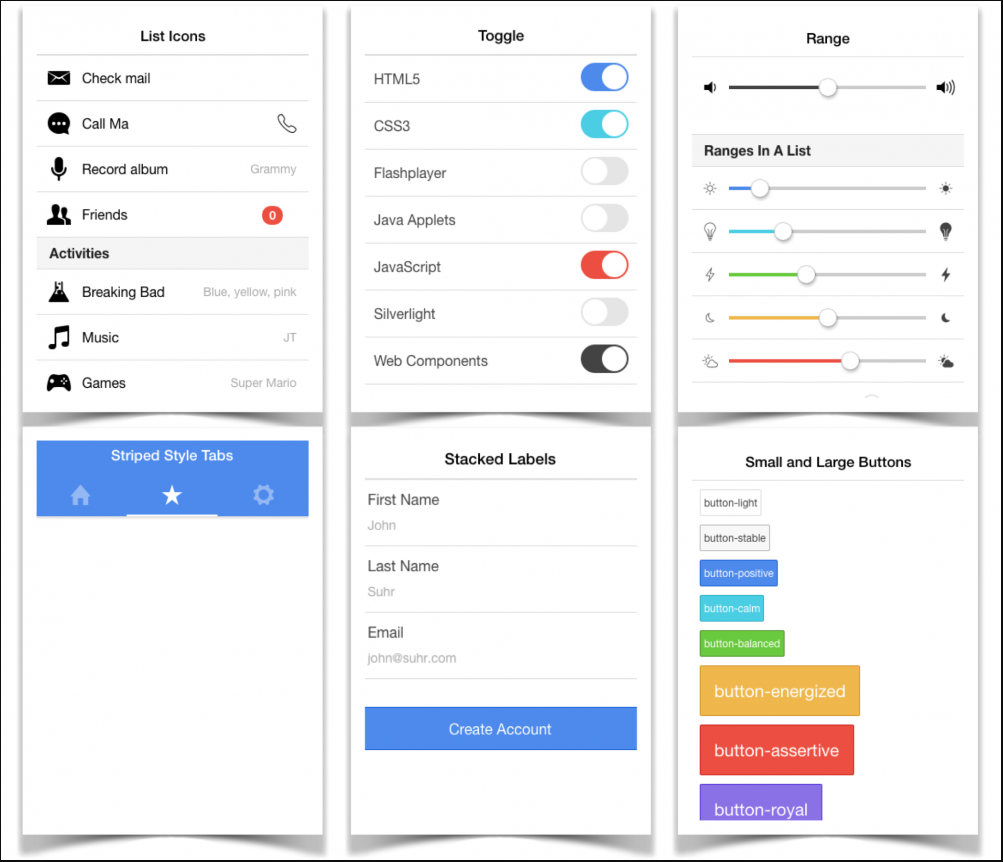
\includegraphics[width=10cm, height=7cm]{img/IonicUI.png}
\caption{Ionic UI.}
\end{figure}

\subsubsection{OS oriented styles}
Ionic is not just a good interface, it is adapted to the specifics of various operating systems and is thought through to the smallest detail. Animations, icons, fonts, all this with the same code will look like the operating system under which the application is built (Android or iOS, and starting with the second version and Windows Phone).\cite{IonicOS}

\subsubsection{Cordova}
Apache Cordova is a platform for developing open source mobile applications. It allows you to use standard web technologies such as HTML5, CSS3 and JavaScript for cross-platform development, avoiding the native development language for each of the mobile platforms. Applications are performed inside a wrapper targeted at each platform and rely on standard APIs to access device sensors, data, and network status. \cite{Cordova}

\begin{figure}[h]
\centering
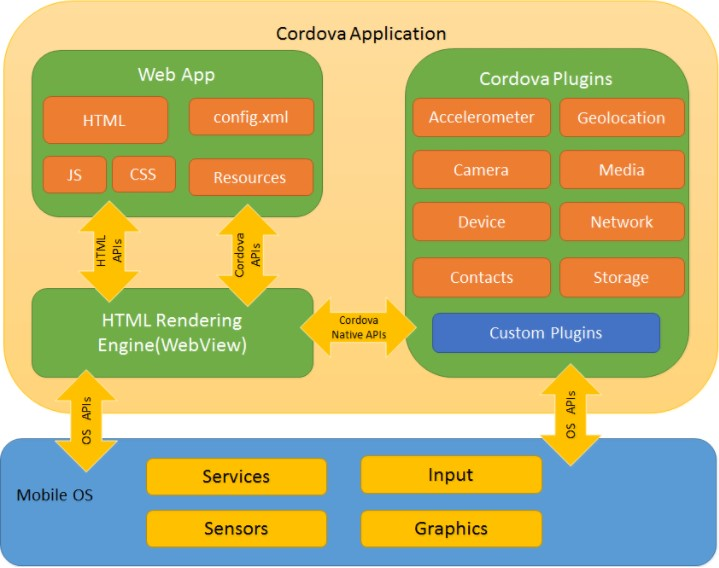
\includegraphics[width=10cm, height=7cm]{img/Cordova.jpg}
\caption{Cordova Application}
\end{figure}

Cordova is a platform that allows you to develop mobile applications on different platforms, by embedding the browser in a mobile application. In fact, your application is a mini-browser that shows one single site - your application. All resources can be placed in the distribution package of the application to accelerate the download, and you can download from the server if necessary.\par
By default, Cordova provides only basic browser capabilities that are available on this mobile device, but it allows you to extend the set of functions available in the browser by using plugins. Each plugin provides a unified interface that can be used from a browser on different platforms. And if the supported CSS / JS functions differently in each browser from the version of the operating system or platform, the Cordova functional tries to provide unified functionality for all supported versions of mobile OS.\par
Even though this approach has its limitations in the form of the need to consider differences in mobile browsers, it still allows you to create high-quality cross-platform applications. \cite{Cordova}

\section{languages}

\subsection{Angular}

\subsection{Typescript}

\subsection{JavaScript}
Javascript is a programming language with which web pages are given interactivity. It creates applications that are included in the HTML-code (for example, questionnaires or registration forms that are filled in by the user).\par The uniqueness of this programming language is that it is supported by almost all browsers and fully integrated with them, and all that can be done with it is done very simply. No other technology accommodates all these advantages together. To date, this technology is actively developing also developing a programming language Javascript2 \cite{JavaScript}

\begin{minted}{js}
// add two numbers
<script>
    var num1, num2, sum
    num1 = prompt("Enter first number")
    num2 = prompt("Enter second number")
    sum = parseInt(num1) + parseInt(num2) // "+" means "add"
    alert("Sum = " + sum)  // "+" means combine into a string
</script>
\end{minted}
\cite{JavaScriptCode}

\subsection{CSS}
CSS (Cascading Style Sheets) - cascading style sheets. In fact, they serve to separate the page structure and its content from its appearance.\par If the page is completely written in HTML, then each element of the code determines not only the content element of the page but also its way of displaying. For example, not only that there is a text "Hello" in such and such a place, but also that this text is highlighted in bold and red.\par With the use of CSS code, everything happens a little differently. With the help of HTML, only the order of the content elements of the page and their classes are described. The corresponding classes are written in the CSS file. Each of them is assigned a set of properties. Now, when we assign a class to an HTML element, then all the properties of this class are applied to it. Do not write all these properties every time. Now, when sites have many pages, you can not do without CSS. \cite{CSS}

\begin{minted}{css}
body {
  font-family: Verdana, 
  Arial, sans-serif;
  }
\end{minted}

\subsection{Tex}

\section{Software and tools used for development}

\subsection{Visual Studio Code}
\cite{VSCode}.

\subsection{Postman}

\subsection{Sharelatex}

\subsection{GitHub}
GitHub hosting project on the Internet. It can be used freely for Open Source projects. Now GitHub is the most popular hosting service for developers. It uses the Git version control system, hence the name GitHub.\par

The project is hosted on GitHub and is called a repository. Anyone can subscribe to an account on GitHub and create their own repositories. GitHub users can add other users to their project to work together.\par

GitHub users have access to other open source projects this enables them to work on it themselves. Developers use this function to send patches and make their own code for other open source projects.\par 

In addition to being just a hosting project, GitHub is also a great social networking site for developers and programmers. It allows users to follow each other, subscribes to project updates, like them, giving them an assessment, etc. These functions allow users to receive updates for projects in which they are interested, or stay in touch with colleagues and employees.\par

GitHub is not only used for programming and software development. It is also used by many other types of projects. For example, open source tutorials, documentation projects, training resources and other projects in which users can work together.\cite{GitHub}\par

Some sample examples of git commands:
\begin{itemize}

    \item git add .\par
    Adds all modified and untracked files in the current directory
    
    \item git commit -m "Commit message"\par
    To commit changes.
    
    \item git push origin master\par
    To send changes to repository. 
\end{itemize}

\subsection{Notpad++}

\chapter{System Design}

In this section, we will cover the overall design and architecture of our Application. We will do this through code snippets and visual aids to help you get a understanding of the Application design. The System design chapter will be broken up into 3 parts representing the 3 tier architecture. Data Tier represented by our Databases Mongo DB and Firebase, Logic Tier represented by NodeJS servers, Presentation Tier which will be represented by Ionic 3.
The image below shows the overview of our Architecture:

\begin{figure}[h]
\centering
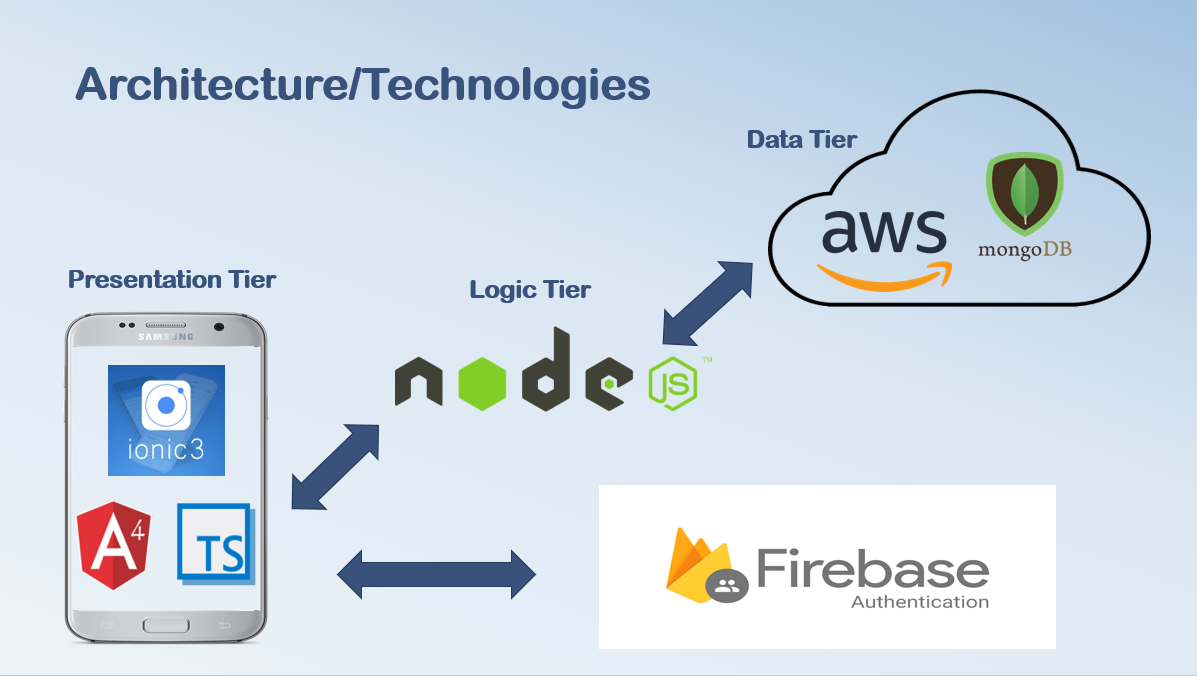
\includegraphics[width=14cm, height=7cm]{img/Architecture}
\caption{System Architecture.}
\end{figure}

\section{Data Tier}

The data tier represents the overall stored data and gives the ability to store, access, update and delete certain data. For our application we have two databases. One database is used to store our user accounts and the other is used to store our users published ads and forum posts.

\subsection{FireBase}
We chose Firebase to handle our user accounts as it was established in the ionic community for being a good database for login and registration functionality.

\subsection{Mongo DB}

We chose Mongo DB to store our clients ads, host ad images and forum messages as it offers a lot of flexibility. When developing a product no matter how much planning one does, requirements can always be subject to change. With this in mind we chose Mongo as it would allow us to change the structure of database as the project evolved. Mongo allows you to download and host your own Mongo DB server for free. This download comes with its own terminal which you can use to query your database which was very effective tool during development.

\subsection{Hosting}

To Host our Mongo DB we used AWS known as Amazon Web Services. AWS provides students with a free account which we have previously used for other project in our course. We created a AWS instance located on a server in Ireland and configured the in-bound and out-bound rules to allow communication between our node server and Mongo DB database. We simply could run our Mongo DB server on our instance by bringing up a terminal and navigating to our Mongo’s bin folder and use the command below:

Mongo bin image 

\subsection{Collections}

Our Mongo DB would be structured into 3 collections.
\begin{itemize}
    \item properties - stores property models 
    \item rooms - stores room models
    \item messages – stores message models 
    \item images – stores and hosts our images
\end{itemize}


Our Mongo DB structures our models as JSON object in each collection. Here is a property JSON object example:

\begin{minted}[linenos,tabsize=2,breaklines]{json}
    {
        "_id": "5aba78dab36ff80e38c85347",
        "UID": "test@gmail.com",
        "AdID": "2ec810ba29cc91c0ffc19913ef75397f",
        "PropertyType": "House",
        "SingleBeds": 3,
        "DoubleBeds": 1,
        "TwinBeds": 0,
        "EnSuite": 0,
        "NoRooms": 4,
        "Eircode": "H951CF",
        "Address": "Galway city ",
        "LocationDes": "City Suburbs",
        "Price": 2300,
        "Availability": "2018-09-27",
        "Email": "patrickmoran121@gmail.com",
        "Phone": 861234567,
        "Contact": "Phone",
        "Description": "Description house here",
        "Parking": "Yes",
        "Date": "2018-03-27T17:01:14.403Z",
        "__v": 0,
        "ImagesUrl": [
            "http://54.73.1.214:3000/images/5aba78d836ceeb168c045761"
        ],
        "College": [
            "GMIT",
            "NUIG"
        ]
    },
\end{minted}

I will cover how we connect Mongo DB to our NodeJS server in the next section.

\section{Logic Tier}

Logic tier refers to your apps business logic. It his here we program your applications ability to manipulate data. These include creation, storing , updating and deletion of Data. To handle our business logic we use NodeJS. NodeJS was the obvious choice for our 3 tier architecture not only does it link up well with our Mongo DB  but also is easily integrated with our Ionic 3 presentation tier. NodeJS with its light-weight nature and its scalability due to its non-blocking I/O calls allowing tens of thousands of concurrent connections made it more than capable for our application.

Using Java script for our logic tier and using type-script for our providers in our presentation tier made it really easy to transition between the two because of their similarities. For our Logic tier we host two NodeJS servers on our AWS account. Our digs server would handle our ad data and our images server would take care of saving and hosting our images.

\subsection{Connecting the Data Tier}

For creating the connection between the Data Tier and the Logic Tier we used Mongoose. Mongoose is a JavaScript library which allows us to define a schema with strongly typed data. Mongoose then allows you create models which map to a MongoDB Document via the Models schema definition.\cite{Mongoose}

Not only does Mongoose allow you to define strong data models and the ability to manipulate them before saving, it also offers functions to create an easy connection to your database and to validate, save, delete and query your data. In the code snippets below from our digs server you will find examples of this:
Here we show how we connected to our Database using Mongoose:

\begin{minted}[linenos,tabsize=2,breaklines]{js}
var mongoose = require('mongoose');     
var morgan = require('morgan');             
var bodyParser = require('body-parser');    
var methodOverride = require('method-override'); 
var cors = require('cors');
 
// Configuration
mongoose.connect('mongodb://localhost/digsdb');
\end{minted}

\noindent Here we can see our room data model and how we declare each data type:

\begin{minted}[linenos,tabsize=2,breaklines]{js}
// Models
var Room = mongoose.model('Room', {
    UID: String,
    AdID: String,
    RoomType: String,
	College: [String],
	Address: String,
    Eircode: String,
    LocationDes: String,
    Price: Number,
    Availability: String,
    Email: String,
    Phone: Number,
    Contact: String,
    Description: String,
    Parking: String,
	ImagesUrl: [String],
	Date: Date,
});
\end{minted}

\subsection{Connecting the Presentation Tier}

For the moment we are just dealing with the Logic Tier side. In the Logic tier we have configured our digs server to run on port 8080 and our images server to run on port 3000. It is on these ports where our servers will send and receive traffic to our presentation layer.

Using our IP address, port number and routing address the presentation layer will be able to send http requests to our servers. Depending on the routing address provided will determine what action the server will take on our data tier. In the next section I will go through some of the functions and queries Mongo and Mongoose provide for accessing and querying of data.

\subsection{Routing and Access of Data}

Here we will show some of our routing and mongoose functions which allow to us to query our data tier Mongo DB. \\

Here we can see a Http Get request being performed on our Rooms Collection. This function is accessed though its routing address “/api/rooms” which we will see below:\\

\begin{minted}[linenos,tabsize=2,breaklines]{js}

// Get rooms
app.get('/api/rooms', function(req, res) {

	console.log("fetching rooms");
	Room.find(function( err, rooms) {

		if (err)
			res.send(err)

		res.json(rooms); 
	});
});

\end{minted}


This function will return an array of room objects from the database and send them to our Ionic application in JSON format.\\


In our next function we can see our server performing a POST http request on our Properties collection. As you can see below the function is accessed through a similar routing address “/api/properties” except this time we use app.post rather than get. \\

\begin{minted}[linenos,tabsize=2,breaklines]{js}

// create properties and send back all properties after creation
app.post('/api/properties', function(req, res) {

	console.log("creating properties");
	let d = Number(req.body.DoubleBeds);
	let s = Number(req.body.SingleBeds);
	let t = Number(req.body.TwinBeds);
	let e = Number(req.body.EnSuite);
	total = d + s + t + e;

	Property.create({
		UID: req.body.UID,
		AdID: req.body.AdID,
		PropertyType: req.body.PropertyType,
		SingleBeds: req.body.SingleBeds,
		DoubleBeds: req.body.DoubleBeds,
		TwinBeds: req.body.TwinBeds,
		EnSuite: req.body.EnSuite,
		NoRooms: total,
		College: req.body.College,
		Eircode: req.body.Eircode,
		Address: req.body.Address,
		LocationDes: req.body.LocationDes,
		Price: req.body.Price,
		Availability: req.body.Availability,
		Email: req.body.Email,
		Phone: req.body.Phone,
		Contact: req.body.Contact,
		Description: req.body.Description,
		Parking: req.body.Parking,
		ImagesUrl: req.body.ImageURL,
		Date: req.body.Date,
		done : false
	}, function(err, property) {
		if (err)
			res.send(err);

		Property.find(function(err, properties) {
			if (err)
				res.send(err)
			res.json(properties);
		});
	});

});

\end{minted}

As you can see above we create a Property object with the data received from body of our http request and post to our properties collection. After we do this we then perform a get request and return the new refreshed array of property objects to our Ionic application.\\


We now have shown how we can retrieve and create data from our Mongo DB. Next we shall manipulate existing items in our database through delete and update.\\


Here we demonstrate our delete function on a specific room object in our Rooms collection. As you can see below we use a delete request and our routing address passes through a parameter like so “/api/rooms/room-id”.\\


\begin{minted}[linenos,tabsize=2,breaklines]{js}

// delete a room
app.delete('/api/rooms/:room_id', function(req, res) {
	Room.remove({
		"_id" : req.params.room_id
	}, function(err, room) {

	});
});

\end{minted}


Through this we can remove the room object using the mongoose remove function and the rooms unique identifier passed through in the parameter.\\

Next we show our Update function, here we use a put request. To perform this action we receive the object ID we wish to update as a parameter and also receive the new updated object from the body of the http request.\\


\begin{minted}[linenos,tabsize=2,breaklines]{js}

// update Room ad
app.put('/api/rooms/:UID', function(req, res) {
	
	let UID = req.body.UID;
	
	Room.remove({
		"_id" : req.params.UID
	}, function(err, room) {

	});
	
	Room.create({
		UID: req.body.UID,
		AdID: req.body.AdID,
		RoomType: req.body.RoomType,
		College: req.body.College,
		Eircode: req.body.Eircode,
		Address: req.body.Address,
		LocationDes: req.body.LocationDes,
		Price: req.body.Price,
		Availability: req.body.Availability,
		Email: req.body.Email,
		Phone: req.body.Phone,
		Contact: req.body.Contact,
		Description: req.body.Description,
		Parking: req.body.Parking,
		ImagesUrl: req.body.ImageURL,
		Date: req.body.Date,
		done : false
	}, function(err, room) {
		if (err)
			res.send(err);

		Room.find(function(err, rooms) {
			if (err)
				res.send(err)
			res.json(rooms);
		});
	});
});

\end{minted}


After updating the object we do the same as our previous POST request and perform a get request on our Room collection in order to return the new refreshed array of room objects to our Ionic application.\\


Finally we have our search function. I will show an example below of searching for a property using the following criteria: College, Number of Rooms, Parking and Price.\\


\begin{minted}[linenos,tabsize=2,breaklines]{js}

//search function on college parking price and number of rooms properties
app.get('/api/searchProperties/:col/:numRooms/:parking/:price', 

function(req, res) {
	let Col = req.params.col;
	let numRooms = req.params.numRooms;
	let Parking = req.params.parking;
	let Price = req.params.price
	console.log("fetching Search properties" + Col + numRooms);

	Property.find({"College": Col, "NoRooms":numRooms, "Parking": Parking, "Price": {$lt: Price }}, function(err, properties) {

		if (err)
			res.send(err)

		res.json(properties); 
	});
});

\end{minted}


As we can see above we perform another GET request but this time we take a list of parameters in our routing address in order to search our Properties collection. Using these and our mongoose find function we can search for property objects fitting the criteria passed through. For example : A property that is located beside GMIT, has 4 bedrooms, has no Parking and Price is less than 1200.\\

Here concludes our Logic Tier, next we will discuss our Presentation Tier.

\section{Presentation Tier}

In the Presentation Tier we will cover 3 sections. Firstly we will explain the Ionic 3 app structure, Secondly we will go through our Providers which we use to interact with our NodeJS server and through that our Mongo DB and finally we will go through each of our Digs Apps Pages, displaying what it looks like and its functionality.\\

\subsection{Ionic 3 App Structure}

\noindent Lets get started with the Ionic 3 Apps Structure. In the Figure 5.2 we can see the structure of our Ionic App.

\begin{figure}[h]
\centering
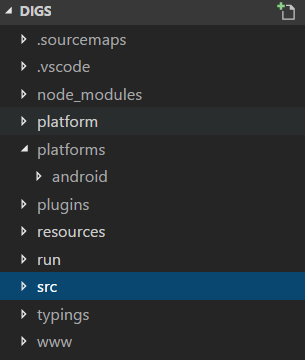
\includegraphics[width=6cm, height=7cm]{img/IonicStructure}
\caption{Ionic 3 Structure.}
\end{figure}


\noindent We will briefly explain each of the main folders and files:

\begin{itemize}
\item Node-modules – Here contains the packages required to run and develop this ionic App
\item Platform – Here contains the technologies needed for a ionic. Ie CSS, JavaScript, Angular
\item Platforms – Here contains the platforms which our Application is being made for. Ie IOS or Android
\item Plugins – Here contains the plugins needed to give the capability to interact with the phones native capabilities.
\item Resources – Here contains the Apps resources such as images, splashscreens and readMe
\item Run – Run enables us to run our application
\item WWW – Here is where our index.html lies and is the root component where the app will load. 
\item Src – This is the folder where we will do most of our coding for our Ionic 3 app. In here we will be using scss, typescript, angularjs and java script.
\end{itemize}

In the src folder Ionic 3 have structured our components into well thought out Folders as seen in figure 5.3 below.

\begin{figure}[h]
\centering
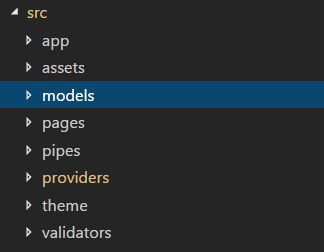
\includegraphics[width=5cm, height=5cm]{img/srcStructure}
\caption{System Architecture.}
\end{figure}

\begin{itemize}
\item App – This is where we set up the base of our app. In here we provide access to components(such as other pages, providers, bootstrap etc) for various pages in our App as well as creating the App shell. For example whether our App will be a side Menu Application structure.
\item Assets – This contains our images and icons. 
\item Models – In here we create our object models. For example our User Model which is made up of a String Email and a String Password.
\item Pages – This is where the majority of our presentation tier code goes. Here we design each of our pages and its functionality. We will be going into each page in more detail below.
\item Pipes – In our pipes folder we link up with our list arrays to perform a search depending on price of a accommodation.
\item Providers – This is where we link our Application to our Logic Tier Servers. We have 4 providers handling our messages, images, properties and rooms. In the next section we will show you how we accomplish this.
\item Theme – Theme allows us to set the over all design and look of our app through global scss.
\item Validators – In here we provide functions to validate whether users input was correct. Ie valid email address.
\end{itemize}

\subsection{Providers}

Providers gives our Application access to our data tier through our servers. In here we provide the logic and perform http requests to our NodeJS Servers to either return , create , update or delete data. Rather than repeating ourselves for each provider we will give examples of how our provider works using the RoomAd.ts Provider.




\chapter{System Evaluation}
This Chapter evaluate the application
\begin{itemize}
    \item Scalability
    \item Robustness
    \item Maintainability
    \item Extensibility
\end{itemize}

\par \textbf{Scalability:} 

\par \textbf{Robustness:}.

\par \textbf{Maintainability:}

\par \textbf{Extensibility:} T

\section{Testing}

\section{Outcomes VS. Objectives}

\section{Limitations}

\section{Opportunities}

\chapter{Conclusion}


\begin{itemize}
\item A Test

\item A Test2
\item A Test3
\end{itemize}
A Test4
\section{Future Development}

\chapter{Appendix}

\textbf{Project Source Code Link: }link to github \\
\textbf{Project Documentation Link: } \\

